%%% Local Variables: 
%%% mode: latex
%%% TeX-master: t
%%% End: 

\documentclass[a4paper, 12pt]{article}
\usepackage{graphicx}
\usepackage{amsmath}
\usepackage[T1]{fontenc}		% F�r svenska bokst�ver
\usepackage[swedish]{babel}
\usepackage{listings}


\title{TDTS07 Lab Report 3}
\author{Nora Björklund and Christopher Hallberg}
\begin{document}
\maketitle


\section{Simulation-based design space exploration for energy minimization}
\section{Communication in MPSoCs}
\section{Mapping and Scheduling}
\subsection{Scheduling exercise}
In this assignment, since nothing else was given we assume that the
proessors run at the same frequency and that the transfer time between
them is zero.
\begin{figure}[h]
  \centering
  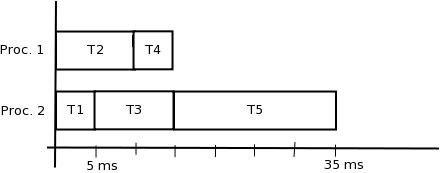
\includegraphics{taskSchedule.png}
  \caption{Task schedule}
  \label{fig:schedule}
\end{figure}
 This can also be confirmed as the minimal execution time since worst
 case propagation time is 35 ms. 

\subsection{Extract execution times for the GSM codec}

\begin{table}[h]
  \centering
  \begin{tabular}{r c c}
    \hline
    Task & First run (cycles) & Second run (cycles) \\
    \hline
    Init & 6002  & X \\
    GetInputAudio & 4576  & 4726 \\
    Preprocess & 14480  & 14258  \\
    LPC\_Analysis & 51759  & 50138 \\
    ShortTermAnalysisFilter & 92101 & 92035 \\
    LongTermPredictor2 &64820&67037\\
                       &66932&68269\\
                       &66262&67599\\
                       &66085&67093\\
    RPE\_Encoding2 &11552&11374\\
                   &10705&10632\\
                   &10667&10623\\
                   &10675&10666\\
    Add2 &1431&1445\\
         &1319&1319\\
         &1319&1319\\
         &1319&1319\\
    Encode & 3364 & 2818 \\
    Output & 3634 & 3522 \\
  \end{tabular}
  \caption{Execution times for GSM Encoder}
\end{table}


\begin{table}[h]
  \centering
  \begin{tabular}{r c c}
    \hline
    Task & First run & Second run \\
    \hline
    Init & 6086 & X \\
    GetInputAudio &1151 & 1129\\
    Decode & 2722& 2540\\
    RPE\_Decoding2 &2793&2232\\
                   &3099&3078\\
                   &3015&3015\\
                   &2979&2979\\
    LongTermSynthesis2 &4790&4608\\
                       &4608&4608\\
                       &4608&4608\\
                       &4580&4580\\
    ShortTermAnalysisFilter & 109882 & 108185\\
    PostProcessing & 7470& 7106\\
    Output & 16631& 16575\\
  \end{tabular}
  \caption{Execution times for GSM Decoder}
\end{table}


\end{document}
